\subsubsection{Interleave}
Pour diminuer les effets NUMA, nous pouvons utiliser la politique d'allocation interleave.
%
Cette politique va distribuer uniformément les pages mémoires sur les différents bancs NUMA.
%
Nous allons donc augmenter la bande passante mémoire en ne modifiant que la latence mémoire moyenne.
%
Sur Rostand, nous obtenons un gain de performance d'environ 20~\% mais les performances sont toujours en dessous des performances obtenues en mémoire partagée (Fig.~\ref{fig:res_spmv_interleave_rostand}).

%   (-_-)   %
\begin{figure}
  \centering
  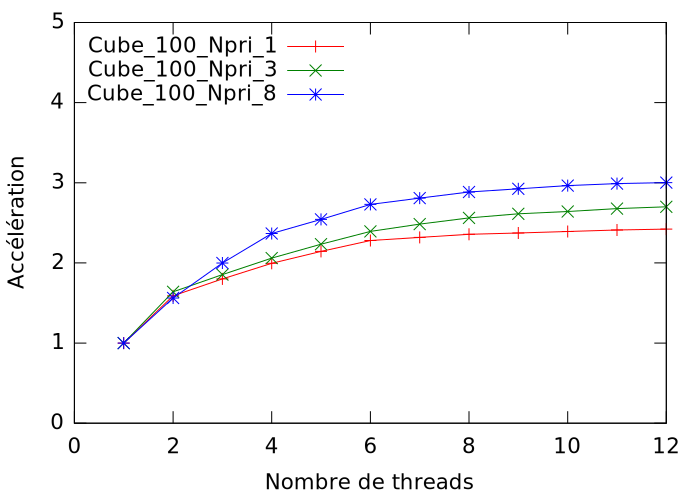
\includegraphics[width=0.7\textwidth]{res_spmv_interleave}
  \caption{Accélération du produit matrice vecteur creux sur Rostand en mémoire partagée avec une politique d'allocation interleave.}
  \label{fig:res_spmv_interleave_rostand}
\end{figure}

Sur Manumanu, on obtient de bons résultats jusqu'à 16 coeurs (Fig.~\ref{fig:res_spmv_interleave_manumanu}).
%
Au delà, nous commençons à utiliser le SGI$^\registered$ NUMAlink$^{\rm TM}$\cite{numalink} et les temps de latence des accès mémoire augmentent.
%
En effet, la majorité des accès mémoire se font sur des bancs NUMA distant.
%
Au final, les résultats de l'allocation interleave sur Manumanu sont proches des résultats de l'allocation first touch.
%
Ce n'est donc pas la bonne solution pour exploiter les performances de cette machine.

%   (-_-)   %
\begin{figure}
  \centering
  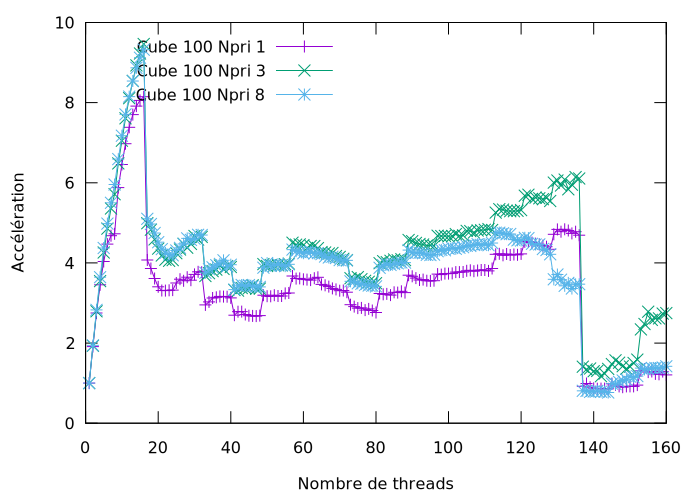
\includegraphics[width=0.7\textwidth]{res_spmv_interleave_manu}
  \caption{Accélération du produit matrice vecteur creux sur Manumanu en mémoire partagée avec une politique d'allocation interleave.}
  \label{fig:res_spmv_interleave_manumanu}
\end{figure}
